\chapter[Proposta]{Proposta}\label{ch:proposta}
  Este capítulo tem como objetivo discutir a solução utilizada durante o
desenvolvimento, assim como os resultados obtidos durante a realização do mesmo. Dentre estes
resultados, estão presentes as fontes de erros levantadas com a experiência do desenvolvimento,
suas respectivas correções, dentro do possível, e a análise da viabilidade da utilização do
sistema no contexto da reabilitação motora. Desse modo, este
capítulo está dividido nas seções: Solução(\ref{sol:solucao}) e Fontes de erro(\ref{sol:fontesErro}).

\section{Solução}\label{sol:solucao}
  Nesta seção serão apresentadas as features envolvidas na solução do sistema,
além das ferramentas usadas. Esta será dividida em Arquitetura (\ref{sub:arquitetura}), Funcionalidades-\textit{features}(\ref{sub:solFeatures}) e
ferramentas(\ref{sub:solFerramentas}).

\subsection{Arquitetura}\label{sub:arquitetura}
  Dentro do Unity 3d não há uma arquitetura específica, isso fica a cargo dos desenvolvedores. Porém podemos dividir o trabalho no unity em duas partes,
a primeira é a parte de vizualização, onde ele desponibiliza um espaço 3d para a inserção dos \textit{gameObjects} e criação das cenas. Um projeto pode
ter mais de uma cena e uma cena pode conter vários \textit{gameObjects}. A segunda é com os chamados \textit{scripts}, que são os códigos que podem
ser adicionados em um \textit{gameObject} dando-lhe a lógica de como se deve comportar durante uma cena de um projeto. Esses códigos podem ser escritos
nas linguagens \textit{javascript} e em C\#.

  Para o desenvolvimento do sistema, podemos ver o diagrama de classe \ref{diagramaClasse}.

  A arquitetura dos scripts ficou um pouco focada na classe \textit{KinectManager} pois ela é a responsável pela comunicação com o kinect.
Abaixo falaremos um pouco sobre o papel de cada classe:

\begin{itemize}
  \item \textit{\textbf{KinectManage}} : Classe responsável pela comunicação com o kinect;
  \item \textit{\textbf{GetCsv}} : Classe responsável por fazer o parser do arquivo csv do movimento desejado;
  \item \textit{\textbf{AvatarController}} : Classe responsável por passar o movimento do usuário para o avatar;
  \item \textit{\textbf{StoredMovimentAvatarController}} : Classe responsável por movimentar o avatar de acordo com o movimento parseado;
  \item \textit{\textbf{GetJointPosition}} : Classe responsável por escrever as posições de todas as juntas e exportar para csv;
  \item \textit{\textbf{KinectGesture}} : Classe com alguns gestos;
  \item \textit{\textbf{KinectWrapper}} : Classe que detém as várias estruturas e importações dll;
  \item \textit{\textbf{KinectManage}} : Classe responsável por guardar as informações dos movimentos parseado;
\end{itemize}


  \begin{figure}[!h]
  \centering
  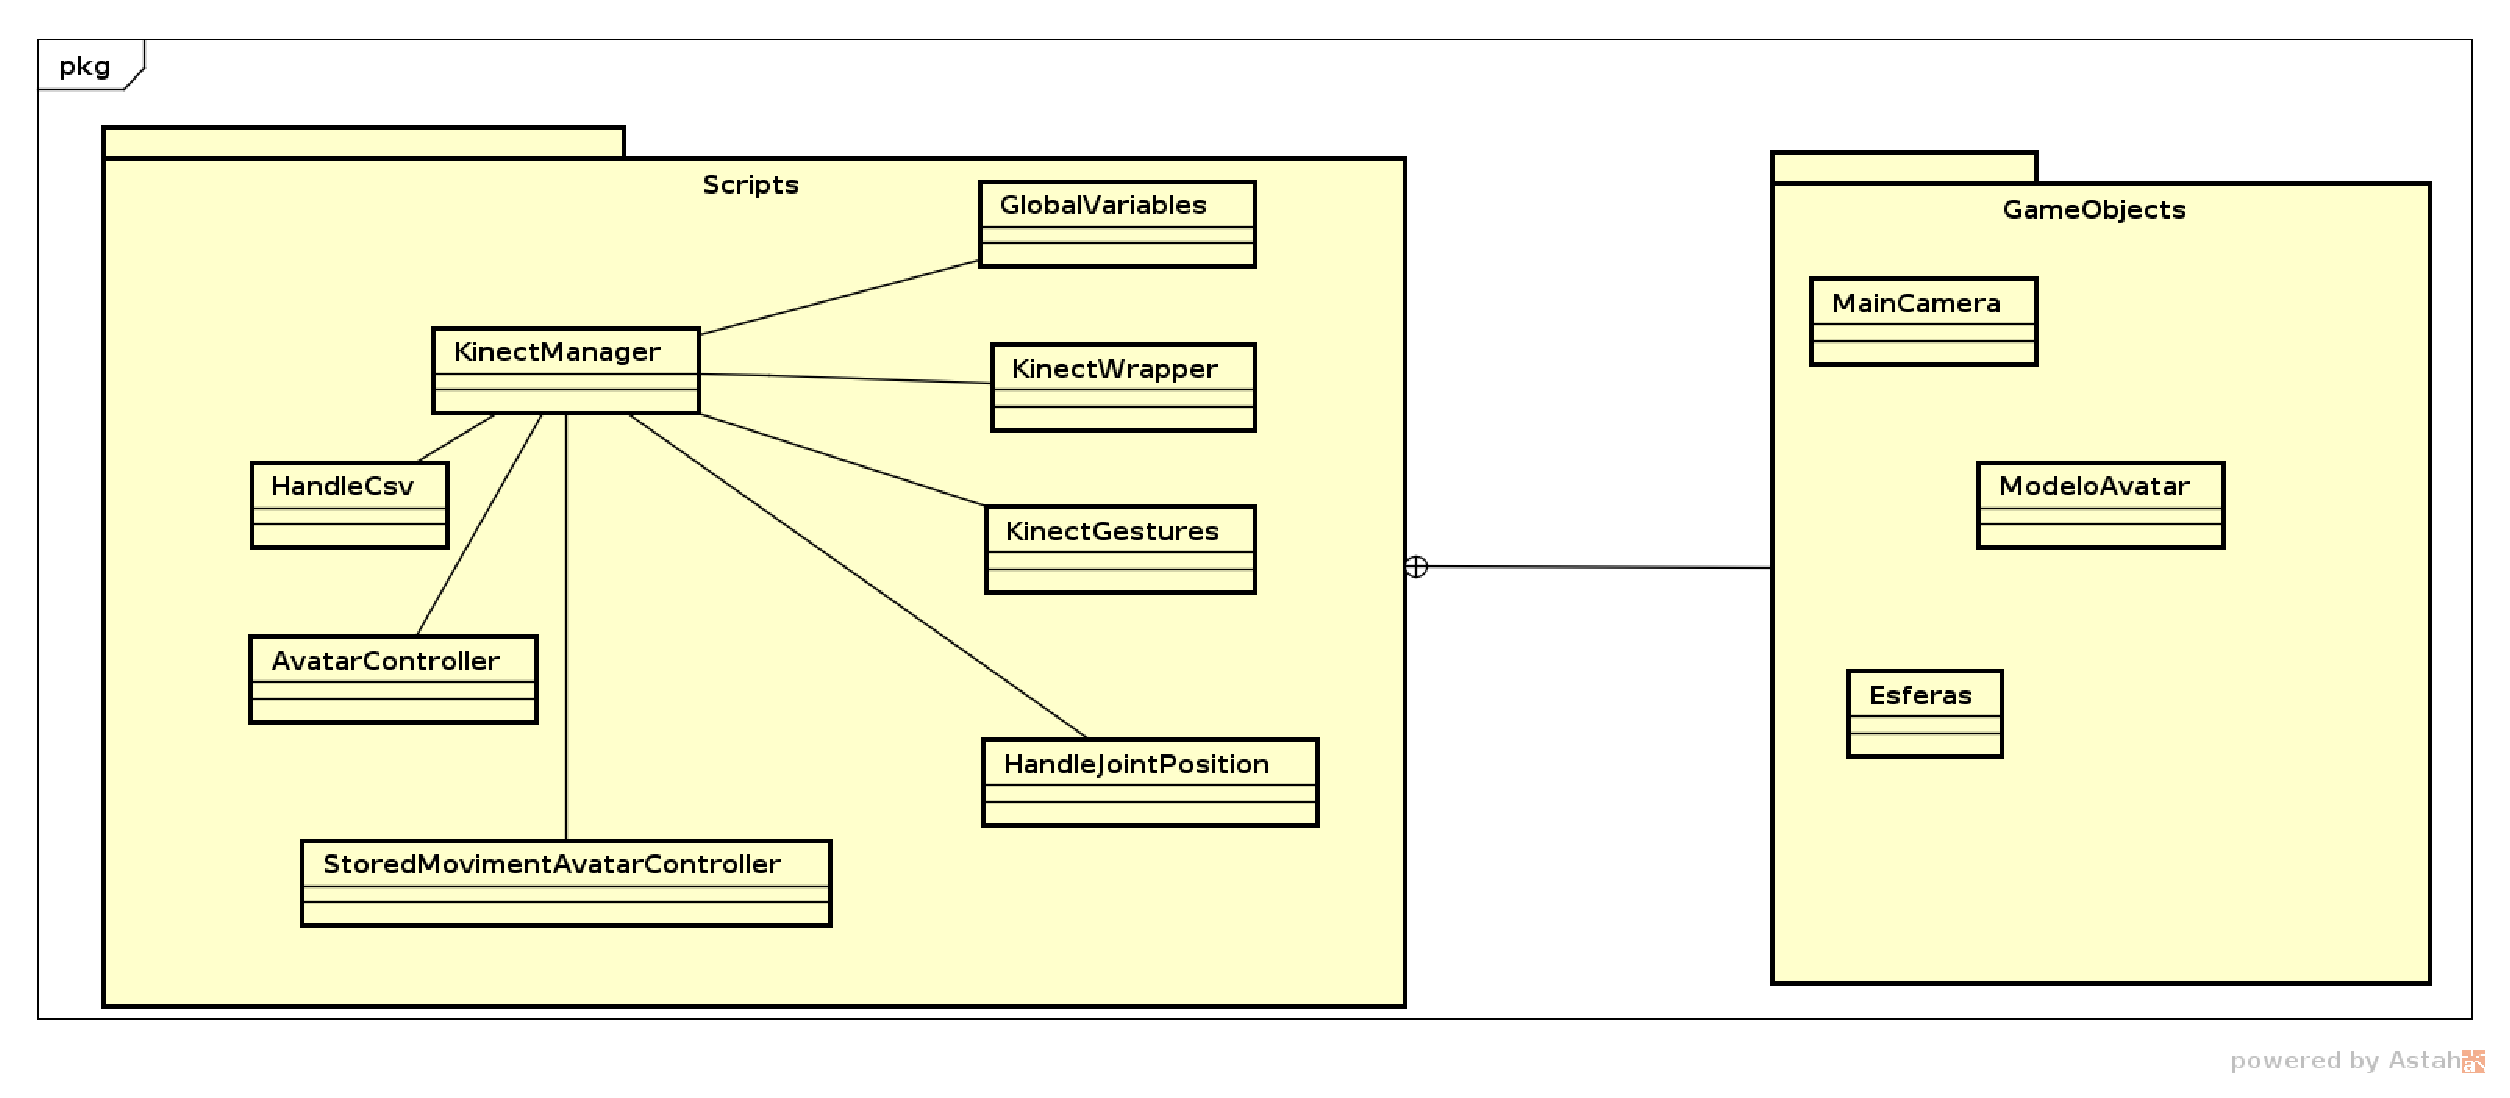
\includegraphics [keepaspectratio=true,scale=0.45]{figuras/DiagramaDeClasse.eps}

  \caption{Diagrama de classe referente ao sistema}
  \label{diagramaClasse}
  \end{figure}


\subsection{\textit{Features}}\label{sub:solFeatures}
  O sistema possui três features, gravação de movimento, leitura de arquivo do movimento desejado e análise da repetição do movimento, elas estão
detalhadas em Funcionalidades do sistema(\ref{sub:features}).

\subsection{Ferramentas}\label{sub:solFerramentas}
  Para o desenvolvimento do sistema foram usadas diversas ferramentas, a seguir serão apresentadas junto
dos artefatos gerados.

\subsection{GIT}\label{sub:git}
  A ferramenta GIT\footnote{https://git-scm.com/} foi desenvolvida por Linus Torvalds, mesmo criador do Linux,
sendo uma ferramenta \textit{open-source}. Disponibiliza uma eficiente forma de versionamento de códigos e
gerenciamento de projetos.

\subsection{Github}\label{sub:github}
  O Github\footnote{https://github.com} é uma ferramenta utilizada para hospedagem remota de projetos GIT.
  A ferramenta contempla uma \textit{Wiki} para documentação do projeto e sistemas de \textit{Issues} e
  \textit{Milestones}\footnote{https://guides.github.com/features/issues/} para gerenciamento de atividades.
Neste trabalho o Github foi utilizado para hospedar a versão escrita do documento e pode ser acessado \href{https://github.com/ricardogtx/Tcc}{aqui}.

Para versionamento do código, foi utilizado o \textit{gitlab} para versionamento do código
e pode ser acessado \href{https://gitlab.com}{aqui}, e o \textit{github} que pode ser acessado \href{https://github.com/ricardogtx/Tcc}{aqui},
para versionamento da versão pdf que foi escrito em \href{https://www.latex-project.org/}{\textit{latex}}, um conjunto de macros para o programa
de diagramação de textos, que se tratam de um repositório de projetos baseado no sistema Git de controle de versão e amb.

\subsection{Gitlab}\label{sub:gitlab}
  O Gitlab\footnote{https://gitlab.com} é outra ferramenta utilizada para hospedagem remota de projetos GIT.
  A ferramenta assim como o Github contempla uma \textit{Wiki} para documentação do projeto e sistemas de \textit{Issues} e
  \textit{Milestones}\footnote{https://guides.github.com/features/issues/} para gerenciamento de atividades. Porém seu diferencial é permitir que um
pequeno projeto possa ser privado, enquanto o Github necessita de alguns critérios. Esta ferramenta foi utilizada para hospedar o código e pode ser acessado
\href{https://gitlab.com/ricardogtx/Tcc}{aqui}.

\subsection{Linux Debian}\label{sub:linuxdebian}
		O sistema operacional utilizado durante este trabalho é o Linux Debian\footnote{https://www.debian.org/} sistema livre
e utilizado, neste projeto, para documentação do trabalho, utilizando a
tecnologia LaTeX(\ref{sub:latex}).

\subsection{Windows}\label{sub:windows}
Sistema operacional da Microsoft 10\footnote{https://www.microsoft.com/pt-br/} , utilizado para implementação do código
por possibilitar configuração simplificada da comunicação entre o \textit{Kinect} e o computador.

\subsection{LaTex}\label{sub:latex}
O LaTeX\footnote{https://www.latex-project.org/} 3.14 é um sistema para criação de documentos utilizando textos \textit{tex},
 foi incialmente desenvolvido por Leslie Lamport, na década de 80. O LaTeX oferece diversos comandos avançados para organização
 de alto nível de documentos, incluindo facilitadores para citações, bibliografias, fórmulas matemáticas, figuras e tabelas.

 \subsection{Visual Studio}\label{sub:codigo}
   Para a edição e criação do código foi usado o Micorosoft Visual Studio\footnote{https://www.visualstudio.com/pt-br/} uma IDE\textit{(Integrated development enviroment)} disponibilizada pela microsoft
e possui apoio para várias linguagens de programação, principalmente C\#.

\subsection{Atom}\label{sub:atom}
		O Atom\footnote{https://atom.io/} é um editor de texto, possui apoio para diversas linguagens de programação, incluindo textos em LaTeX, além de
ter um núcleo hackeável e muito configurável.



\subsection{Diagrama de sequência}\label{sub:diagramaSequencia}
  Consiste em um diagrama que tem o objetivo de mostrar como as mensagens entre os objetos são trocadas no decorrer do tempo para a realização de uma operação.\cite{diagramaSequencia}
Como pode ser visto em \ref{diagramaFisio} e \ref{diagramaPaciente}, existe dois momentos de trocas de mensagens, uma com o usuário como fisioterapeuta e outra
com o paciente.

\begin{figure}[H]
\centering
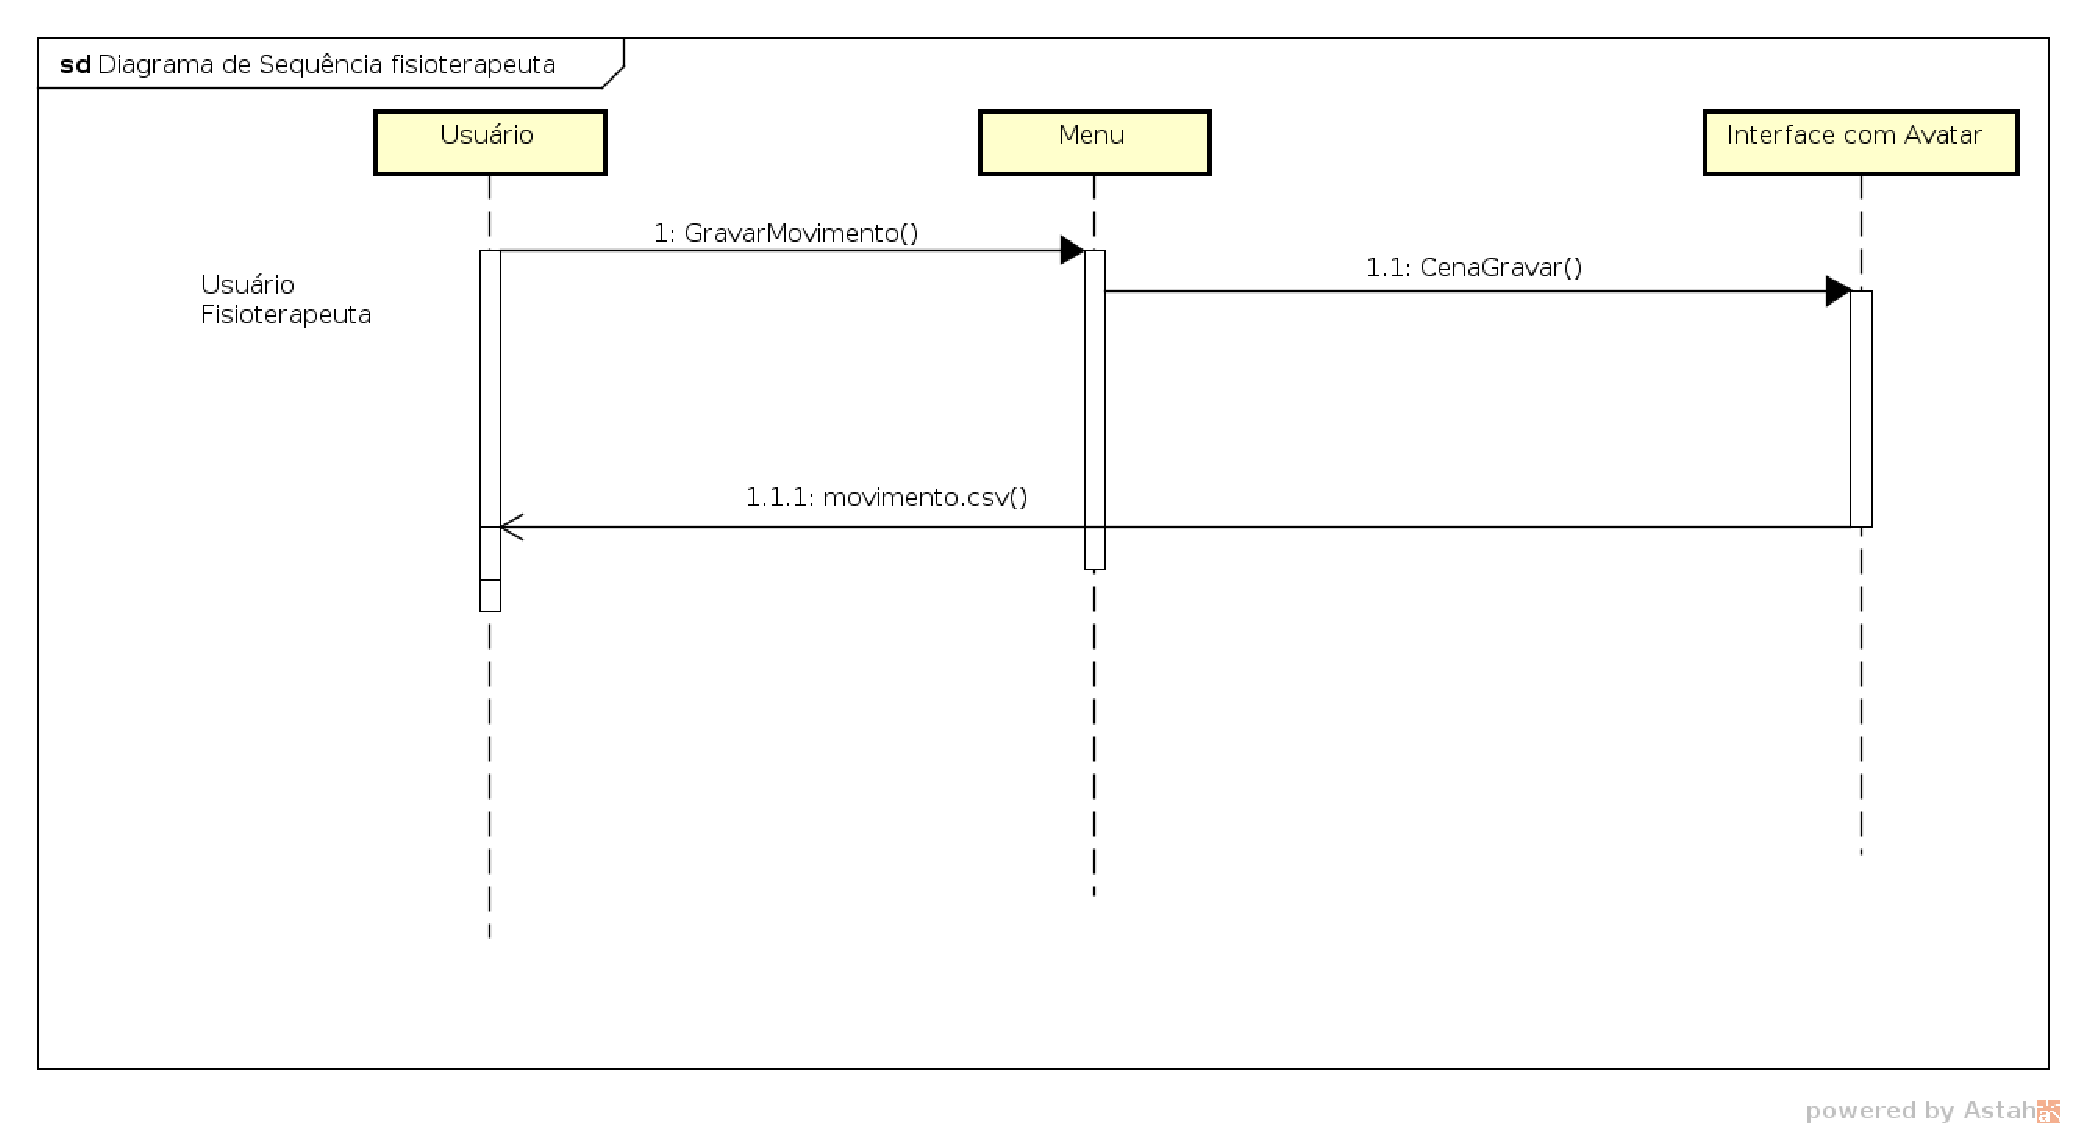
\includegraphics [keepaspectratio=true,scale=0.45]{figuras/diagramaFisio.eps}

\caption{Diagrama de sequência referente ao uso do fisioterapeuta}
\label{diagramaFisio}
\end{figure}


\begin{figure}[H]
\centering
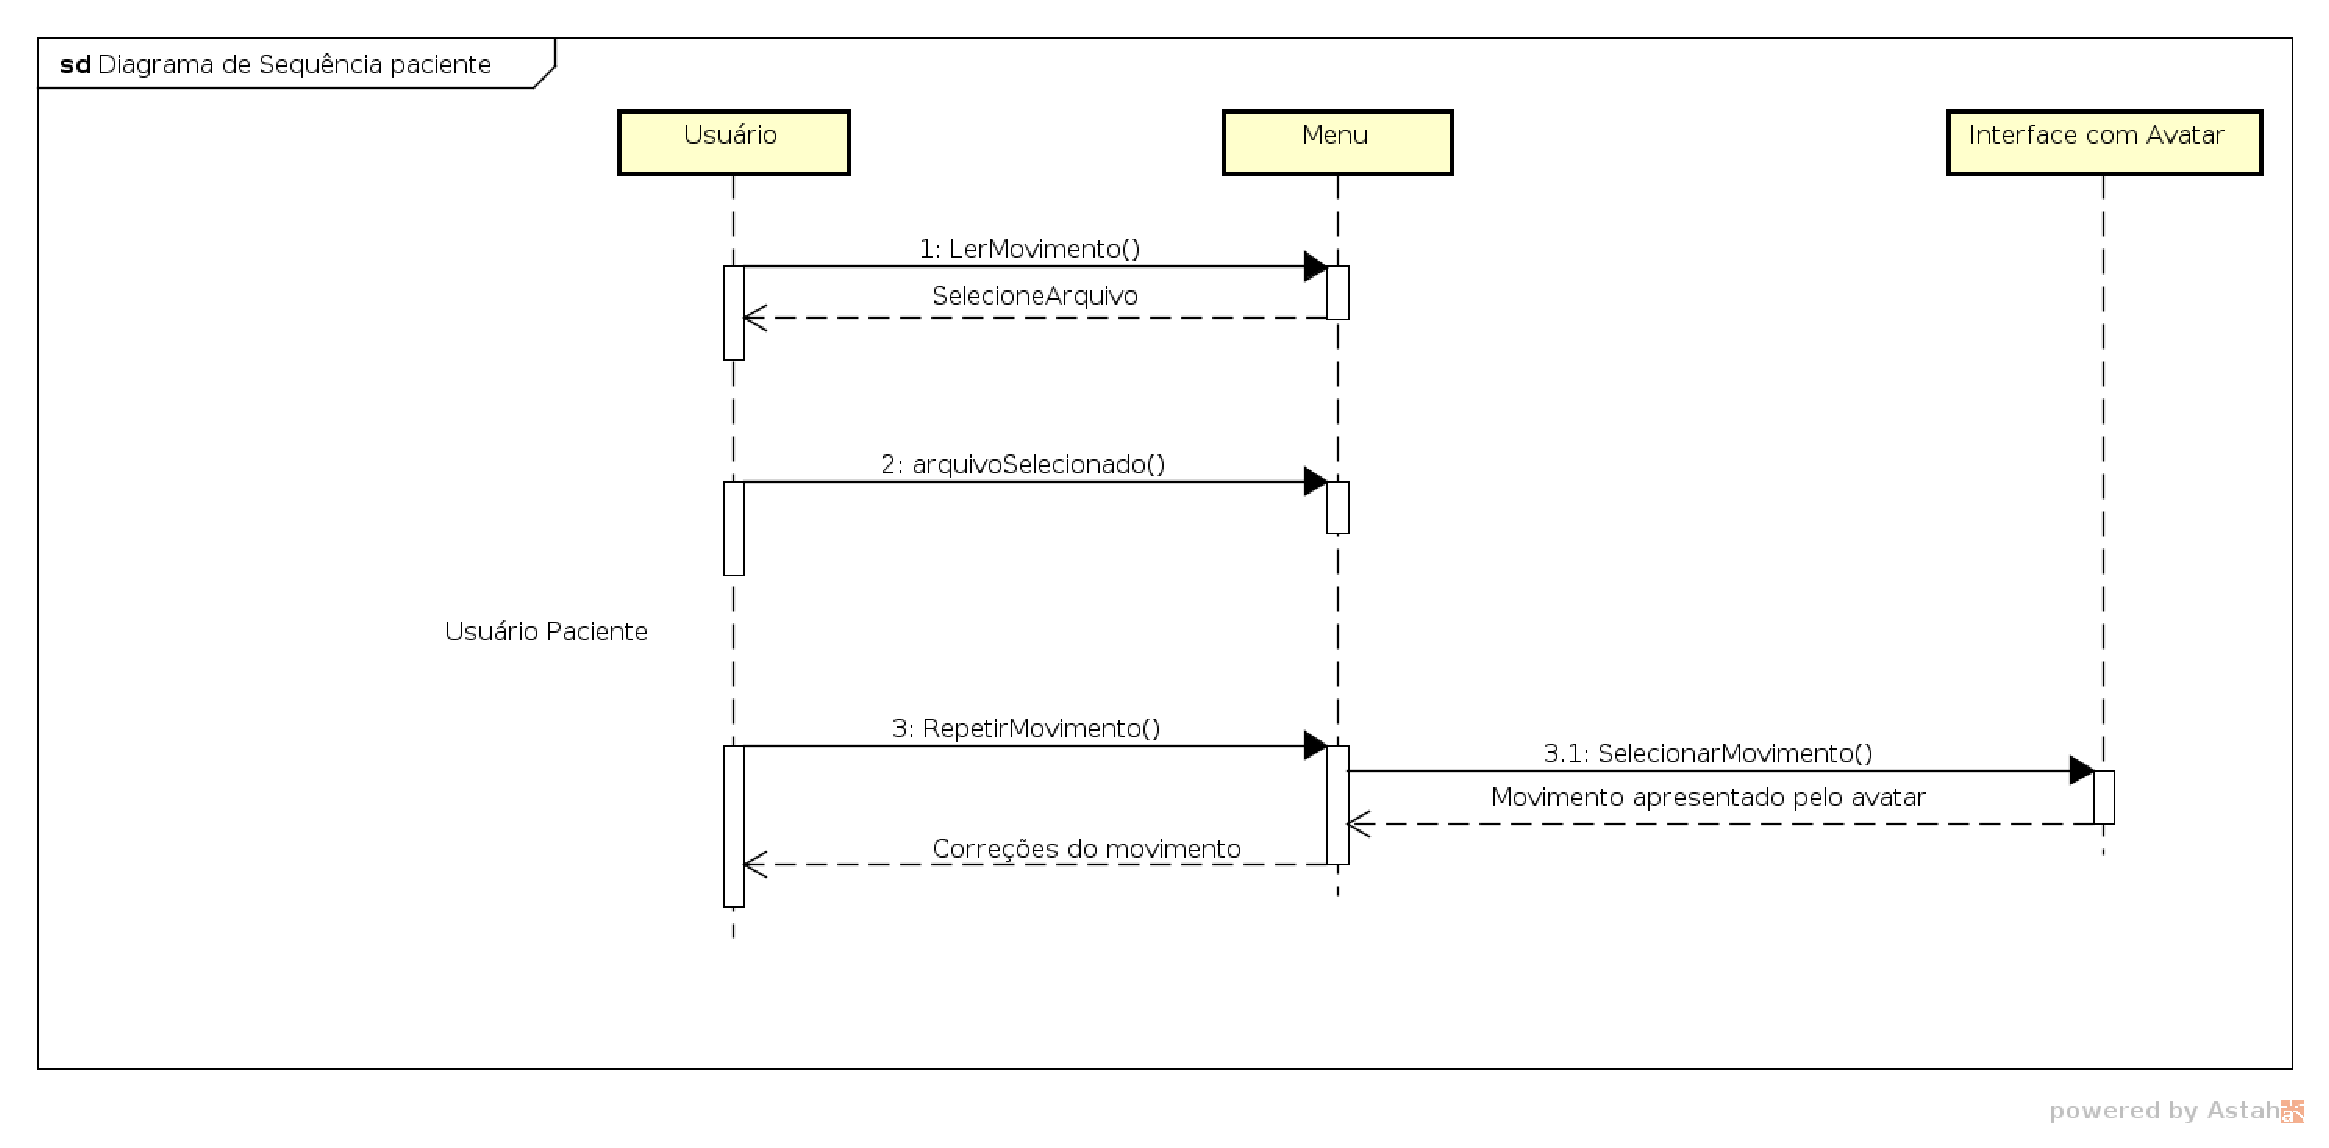
\includegraphics [keepaspectratio=true,scale=0.45]{figuras/diagramaPaciente.eps}

\caption{Diagrama de sequência referente ao uso do paciente}
\label{diagramaPaciente}
\end{figure}

  Para a criação desses artefatos foi utilizado a ferramenta Astah community que pode ser encontrada \href{http://astah.net/download#community}{aqui} gratuitamente.


\subsection{\textit{Kanban}}\label{sub:kanban}
  \textit{Kanban} é um termo de origem japonesa e significa literalmente “cartão” ou “sinalização”.
Este é um conceito relacionado com a utilização de cartões (post-it e outros) para indicar o andamento dos fluxos de produção em empresas de fabricação em série.\ref{sec:kanban}

  Ao longo do desenvolvimento foi utilizado o \textit{trello}  que é uma espécie de \textit{kanban eletrônico}, ele pode ser acessado \href{https://trello.com/}{aqui} gratuitamente.

\section{Fontes de Erro}\label{sol:fontesErro}
  Como dito antes, a principal fonte do erro do sistema é o kinect. Por este motivo, durante a realização do desenvolvimento buscou-se minimizar a margem de erro
do sensor, deixando uma margem de graus sobre o movimento das juntas que não comprometesse de fato o movimento.
